\chapter{Robótica evolutiva}
\label{cha:evolutionary-robotics}

\section{Introdução}

Segundo Nolfi et al. \cite{nolfi1994howtoevolve}, o projeto de um controlador para robôs autônomos apresenta duas grandes dificuldades:

\begin{enumerate}
    \item A coordenação das partes de um robô é extremamente difícil, tanto a nível do sistema de controle quanto a nível mecânico. A imprevisibilidade da interação entre esses dois níveis resulta em mais dificuldades.
    \item Robôs autônomos interagem com um ambiente externo e portanto o modo como esse se comporta determina os estímulos que receberá de entrada. Essa relação introduz um efeito de longo termo difícil de prever e modelar.
\end{enumerate}

Como uma forma de automatizar esse processo, os conceitos de computação evolutiva e seus algoritmos são utilizados para a construção gradual de tais controladores. Daí, a área denominada robótica evolutiva (\textit{Evolutionary Robotics} - ER). Na literatura, Brooks \cite{brooks1992artificiallife} utiliza de programação genética para construir um programa controlador em linguagem de alto nível. Dorigo e Schenepf \cite{dorigo1993geneticsbased} tratam o problema com uso de sistemas classificadores. Hoffmann e Pfister \cite{hoffmann1996evolutionary} utilizam um controlador de lógica difusa. No entanto, a estratégia mais comum \cite{nelson2009fitness} -- e adotada nesse trabalho -- é com o uso de redes neurais artificiais \cite{cliff1992evolvingvisually} \cite{miglino1994selection} \cite{nolfi1994phenotypic}.

A Seção \ref{sec:evolutionary-computation} descreve os quatro algoritmos evolutivos avaliados nesse trabalho. A Seção \ref{sec:ann} descreve as redes neurais artificiais e, mais especificamente, o modelo utilizado para representação do controlador do robô utilizado.

\section{Computação evolutiva}
\label{sec:evolutionary-computation}

A Computação Evolutiva (CE) é uma área da computação focada em métodos de otimização global. Os algoritmos dessa área são estocásticos e utilizam metaheurísticas que, geralmente, modelam fenômenos naturais \cite{michalewicz1995heuristic}. De forma bastante abstrata, são processos que melhoram iterativamente soluções para um determinado problema a partir de um conjunto inicial geralmente aleatório.

Dentre os diversos algoritmos emergentes da computação evolutiva podemos notar alguns: algoritmo genético, programação genética, evolução diferencial, \textit{particle swarm optimization}, \textit{ant colony optimization} etc.

\subsection{Algoritmo genético}

Algoritmos genéticos (\textit{Genetic Algorithms} - GAs) são algoritmos evolutivos cuja heurística baseia-se no processo de evolução natural. Esses algoritmos codificam uma potencial solução para um problema específico em uma estrutura de dados semelhante a um cromossomo e aplica operadores de recombinação a essas estruturas a fim de preservar informação crítica \cite{whitley1994genetic}.

O algoritmo canônico inicia com uma população (geralmente aleatória) de indivíduos. Cada indivíduo representa uma possível solução ao problema e é composto de um ou mais cromossomos. Cada parâmetro da solução é codificado em um gene, ou seja, uma \textit{string} de bits. A união dos vários genes compõem um cromossomo. Em seguida, os indivíduos são avaliados em relação a qualidade desses como uma solução do problema. A função que realiza essa avaliação é chamada função de aptidão ou função de \fitness. A partir do resultado dessa avaliação, os operadores são aplicados a fim de gerar uma nova população.

\begin{algorithm}[h]
    \caption{Pseudocódigo de um algoritmo genético padrão}
    \begin{algorithmic}
        \State $P \gets $ população inicial aleatória
        \State $g \gets 0$
        \While {$g \le $ quantidade máxima de gerações}
            \State \Call{Avalia}{P}
            \State $S \gets$ \Call{Seleção}{$P$}
            \State $P \gets \varnothing$
            \ForEach {par de índividuos $(i_{1}, i_{2})$ em $S$}
                \State $P \gets P \>\> \bigcup \>$ \Call{Cruzamento}{$i_{1}, i_{2}$}
            \EndFor
            \State $P \gets $ \Call{Mutação}{$P$}
            \State $g \gets g + 1$
        \EndWhile
    \end{algorithmic}
\end{algorithm}

O operador \textbf{seleção} escolhe indivíduos para reprodução sexuada (cruzamento) ou assexuada (mutação) \cite{erik2012geneticos}.

O \textbf{cruzamento} gera novos indivíduos (\textit{offspring}) a partir da combinação de dois indivíduos selecionados, mantendo características de ambos. A taxa de cruzamento define a probabilidade de ocorrer o cruzamento entre dois indivíduos selecionados.

A \textbf{mutação} consiste na troca aleatória de alguns bits no cromossomo com probabilidade definida pela taxa de mutação.

\subsection{Algoritmos genéticos paralelos}

Algoritmos genéticos paralelos (\textit{Parallel GAs} -- PGAs) \cite{shonkwiler1993parallel} são variações dos GAs em alguns aspectos centrais aos quais a paralelização pode ser aplicada. Assim, é possível obter melhores resultados em relação a qualidade da solução e também a otimização do uso dos recursos computacionais \cite{erik2012geneticos}.

Os algoritmos genético paralelos podem ser classificados da seguinte forma \cite{cantupaz1998asurvey}:

\begin{itemize}
    \item \textbf{Mestre-escravo}: paralelização do cálculo da função de aptidão (única população).
    \item \textbf{\textit{Fine-grained}}: paralelização dos indivíduos de uma única população com frequente comunicação entre as partes.
    \item \textbf{\textit{Coarse-grained}}: diversas populações paralelas com pouca comunicação entre as partes.
\end{itemize}

Nos algoritmos genéticos paralelos \textit{coarse-grained} (\textit{Coarse-Grained Parallel Genetic Algorithms} - CGPGAs) um arquipélago é um conjunto de populações distintas denominadas ilhas e o processo de troca de indivíduos entre as ilhas é chamado migração. Dois parâmetros importantes são introduzidos: a quantidade de indivíduos que são trocados entre as ilhas (taxa de migração) e a frequência em que essas acontecem.

Outro fator importante a ser observado é a topologia dos arquipélagos, ou seja, as possibilidades de caminho para a migração entre as ilhas. Por exemplo, a Figura \ref{fig:ring} apresenta um arquipélago com topologia em anel onde cada ilha é conectada apenas com a próxima a fim de formar um ciclo. A Figura \ref{fig:barabasi-albert} mostra outro exemplo de topologia baseada no modelo Barabási-Albert \cite{albert2002statistical}.

\begin{figure}[H]
    \centering
    \begin{minipage}{.2\textwidth}
        \includegraphics[width=0.9\textwidth]{figures/ring}
        \subcaption{Topologia em anel}
        \label{fig:ring}
    \end{minipage}%
    \quad\quad\quad\quad
    \begin{minipage}{.35\textwidth}
        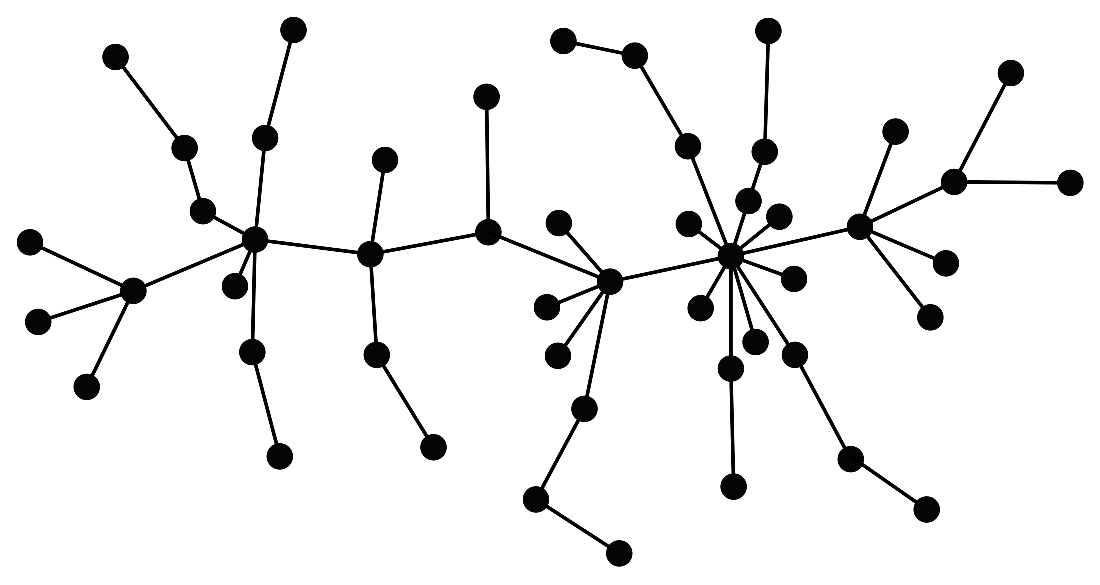
\includegraphics[width=\textwidth]{figures/barabasi-albert}
        \subcaption{Topologia baseada em redes Barabasi-Albert}
        \label{fig:barabasi-albert}
    \end{minipage}

    \caption{Exemplos de topologias de arquipélagos}
\end{figure}

\subsection{\textit{Particle Swarm Optimization}}

O método introduzido por Kennedy e Eberhart \cite{kennedy1995pso} denominado \textit{Particle Swarm Optimization} (PSO) utiliza enxames de partículas para otimização de funções não-lineares. Nesse, para a solução de um problema com $n$ parâmetros, cada partícula $i$ possuí dois vetores $n$-dimensionais: posição $x_{i} = (x_{i1}, x_{i2}, \dots, x_{in})$ e velocidade $v_{i} = (v_{i1}, v_{i2}, \dots, v_{in})$. A cada iteração $t$ ambos os vetores são atualizados da seguinte maneira:

\begin{equation}
\label{eq:pso-vel}
v_{i}^{t} = \omega v_{i}^{t-1} + \alpha \phi (p_{i}^{best} - x_{i}^{t-1}) + \beta \phi (g^{best} - x_{i}^{t-1})
\end{equation}

\begin{equation}
\label{eq:pso-pos}
x_{i}^{t} = x_{i}^{t-1} + v_{i}^{t}
\end{equation}

onde $\phi$ é um número aleatório no interalo $[0,1]$ de distribuição uniforme, $p_{i}^{best}$ é o melhor vetor posição encontrado pela partícula $i$ (localmente) e $g^{best}$ é a melhor posição encontrada por todas as partículas (globalmente).

$\omega$, $\alpha$ e $\beta$ são parâmetros do algoritmo. O parâmetro $\omega$ se traduz em um fator de inércia, ou seja, determina a dependência da velocidade em um momento em relação ao anterior. O nível de confiança nas melhores soluções encontradas localmente e globalmente são determinadas pelos parâmetros $\alpha$ e $\beta$, respectivamente.

\subsection{\textit{Discrete Particle Swarm Optimization}}

Esta variação do PSO difere na representação das partículas. No \textit{Discrete Particle Swarm Optimization} (DPSO) a posição $x_{i} = (x_{i1}, x_{i2}, \dots, x_{in})$ de uma partícula $i$ está contida num espaço discreto e cada elemento do vetor velocidade $v_{ij}$ é um vetor $m$-dimensional contendo as probabilidades de $x_{ij}$ assumir cada um dos $m$ possíveis valores discretos.

Matematicamente,

\noindent\begin{minipage}{.5\linewidth}
$$
P(x_{i,j} = k) = \frac{\sigma (v_{i,j,k})}{S_{i,j}}
$$
\end{minipage}%
\begin{minipage}{.5\linewidth}
$$
S_{i,j} = \sum_{k}^{m} \sigma(v_{i,j,k})
$$
\end{minipage}\\

onde $\sigma$ é a função \textit{sigmoid}, $v$ é o vetor de velocidades e $x$ é o vetor posição.

Desse modo, a probabilidade de $x_{i,j}$ assumir o valor $k$ é determinada pela velocidade $v_{i,j,k}$. Note que $S_{i,j}$ é um coeficiente de normalização e tem a finalidade de permitir que $x_{i,j}$ possa assumir qualquer valor $k$.


\section{Redes neurais artificiais}
\label{sec:ann}

Redes neurais artificias (RNAs) são sistemas computacionais inspirados em sistemas nervosos animais capazes de aprendizado. Matematicamente, RNAs são aproximadores universais \cite{hornik1989universal}. Um RNA é composto por uma rede de unidades de processamento simples (neurônios) que possuem um sinal de saída e podem receber um ou mais sinais de entrada.

\subsection{\textit{Multi-Layer Perceptron}}

Uma rede neural \textit{Multi-Layer Perceptron} (MLP) é composta por uma série de neurônios organizados em camadas, onde cada neurônio recebe, como entrada, a saída dos neurônios da camada anterior. Uma rede com uma camada intermediária é capaz de aproximar qualquer função contínua. Com duas camadas intermediárias, qualquer função pode ser aproximada \cite{cybenko1989mlp}.

\begin{figure}[H]
    \centering
    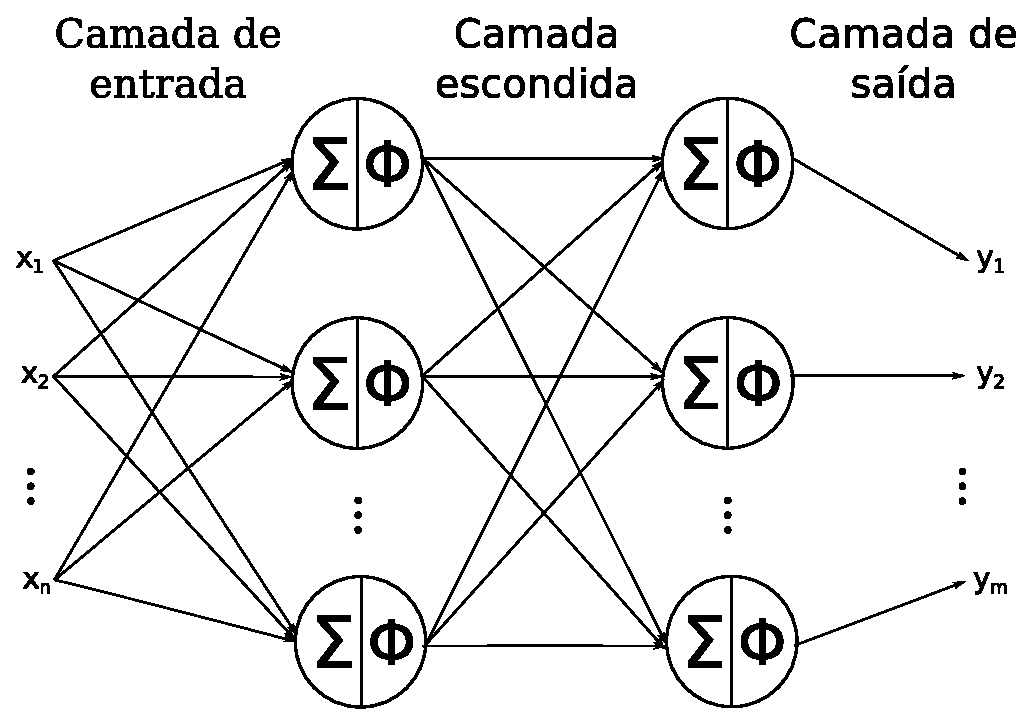
\includegraphics[width=0.5\textwidth]{figures/mlp}
    \caption{Multi-layer Perceptron}
    \label{fig:mlp}
\end{figure}

A saída (y) de um neurônio é determinada pela aplicação de uma função de ativação \(\sigma\) sobre a combinação linear ponderada de todas as suas \(n\) entradas \((x_1, x_2, \dots , x_n)\).

Matematicamente,

\[ y = \sigma ( \sum_{i=1}^{n} w_i x_i ) \]

onde \(w_i\) é um peso associado a entrada \(i\).

Diversas funções pode assumir o papel de função de ativação, sendo as mais comuns:
a função degrau (\ref{eq:degrau}) e a função sigmóide (\ref{eq:sigmoid}).

\begin{equation} \label{eq:degrau}
    \sigma (x) = \left\{
    \begin{array}{l l}
        0 & \quad \text{se } x < 0\\
        1 & \quad \text{caso contrário}
    \end{array} \right.
\end{equation}

\begin{equation} \label{eq:sigmoid}
    \sigma (x) = \frac{1}{1 + e^{-x}}
\end{equation}

É comum encontrar, em cada uma das camadas, um neurônio adicional cuja entrada é sempre \(1\). Este neurônio especial tem o nome de \textit{bias} e a finalidade de deslocar a função de ativação para direita ou esquerda.

O ajuste dos pesos \((w_1, w_2, \dots , w_n)\) é chamado treinamento e existe em duas formas:

\begin{description}
    \item[Supervisionado]: É fornecido ao algoritmo um conjunto de treinamento composto de entradas e suas respectivas saídas. O algoritmo iterativamente ajusta os pesos da rede a fim de que, para cada entrada do conjunto de treinamento, a saída da rede aproximem-se da saída esperada.
    \item[Não supervisionado]: Não demanda conjunto de treinamento, os pesos são ajustados considerando a aptidão da rede à solução do problema.
\end{description}

\subsection{\textit{Time-Delay Neural Network}}
\label{sec:tdnn}

Estendendo os conceitos das redes MLP, uma \textit{Time-Delay Neural Network} (TDNN) permite à cada neurônio armazenar um histórico dos sinais de entrada (Figura \ref{fig:tdnn}). Isto permite que a rede ganhe sensibilidade à padrões temporais, ou seja, a rede pode adaptar-se não só a simples padrões como também a sequências de padrões \cite{kaiser1994tdnn}.

\begin{figure}[H]
    \centering
    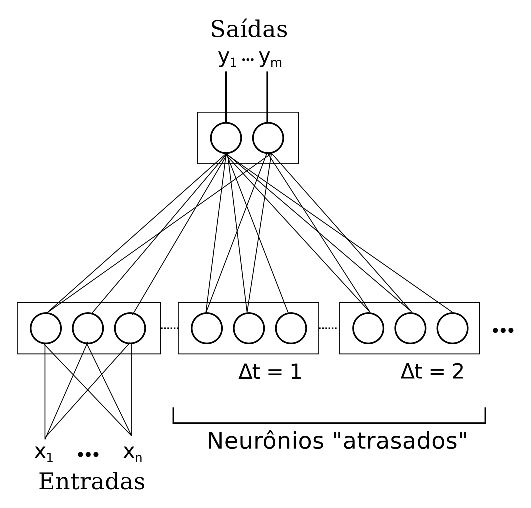
\includegraphics[width=0.5\textwidth]{figures/tdnn}
    \caption{Time-Delay Neural Network}
    \label{fig:tdnn}
\end{figure}